\documentclass[../Main.tex]{subfiles}
\begin{document}

\section{Existing Alternative Games}
\label{chap:existing_games}
In this chapter, seven different alternative games will be presented. The games are picked based on popularity, relevance today, and how they compare to each other. Different types of games are carefully chosen to illustrate the diversity of alternative games that exist. A brief explanation of the game concept and why it is an alternative game will be given in every game section.

\subsection{Hold}
Hold is an application that rewards users for not using their phones \citep{hold_hold_2020}. The game was initially launched in 2016 for iOS and Android, and the primary focus was on Norwegian university students \citep{ringheim_smarttelefon_2018}. Since then, the application’s target group has expanded beyond Norwegian students.

\begin{figure}[H]
    \begin{minipage}{.5\textwidth}
      \centering
      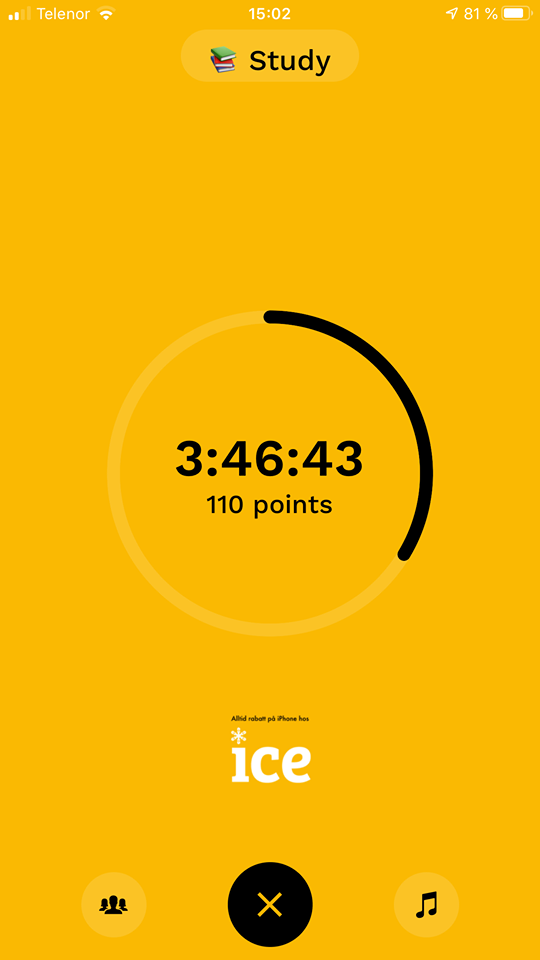
\includegraphics[width=.75\textwidth]{Images/ExistingGames/HoldApp.png}
      \captionof{figure}{Main timer screen in Hold.}
      \label{fig:hold_timer}
    \end{minipage}
    \begin{minipage}{.5\textwidth}
      \centering
      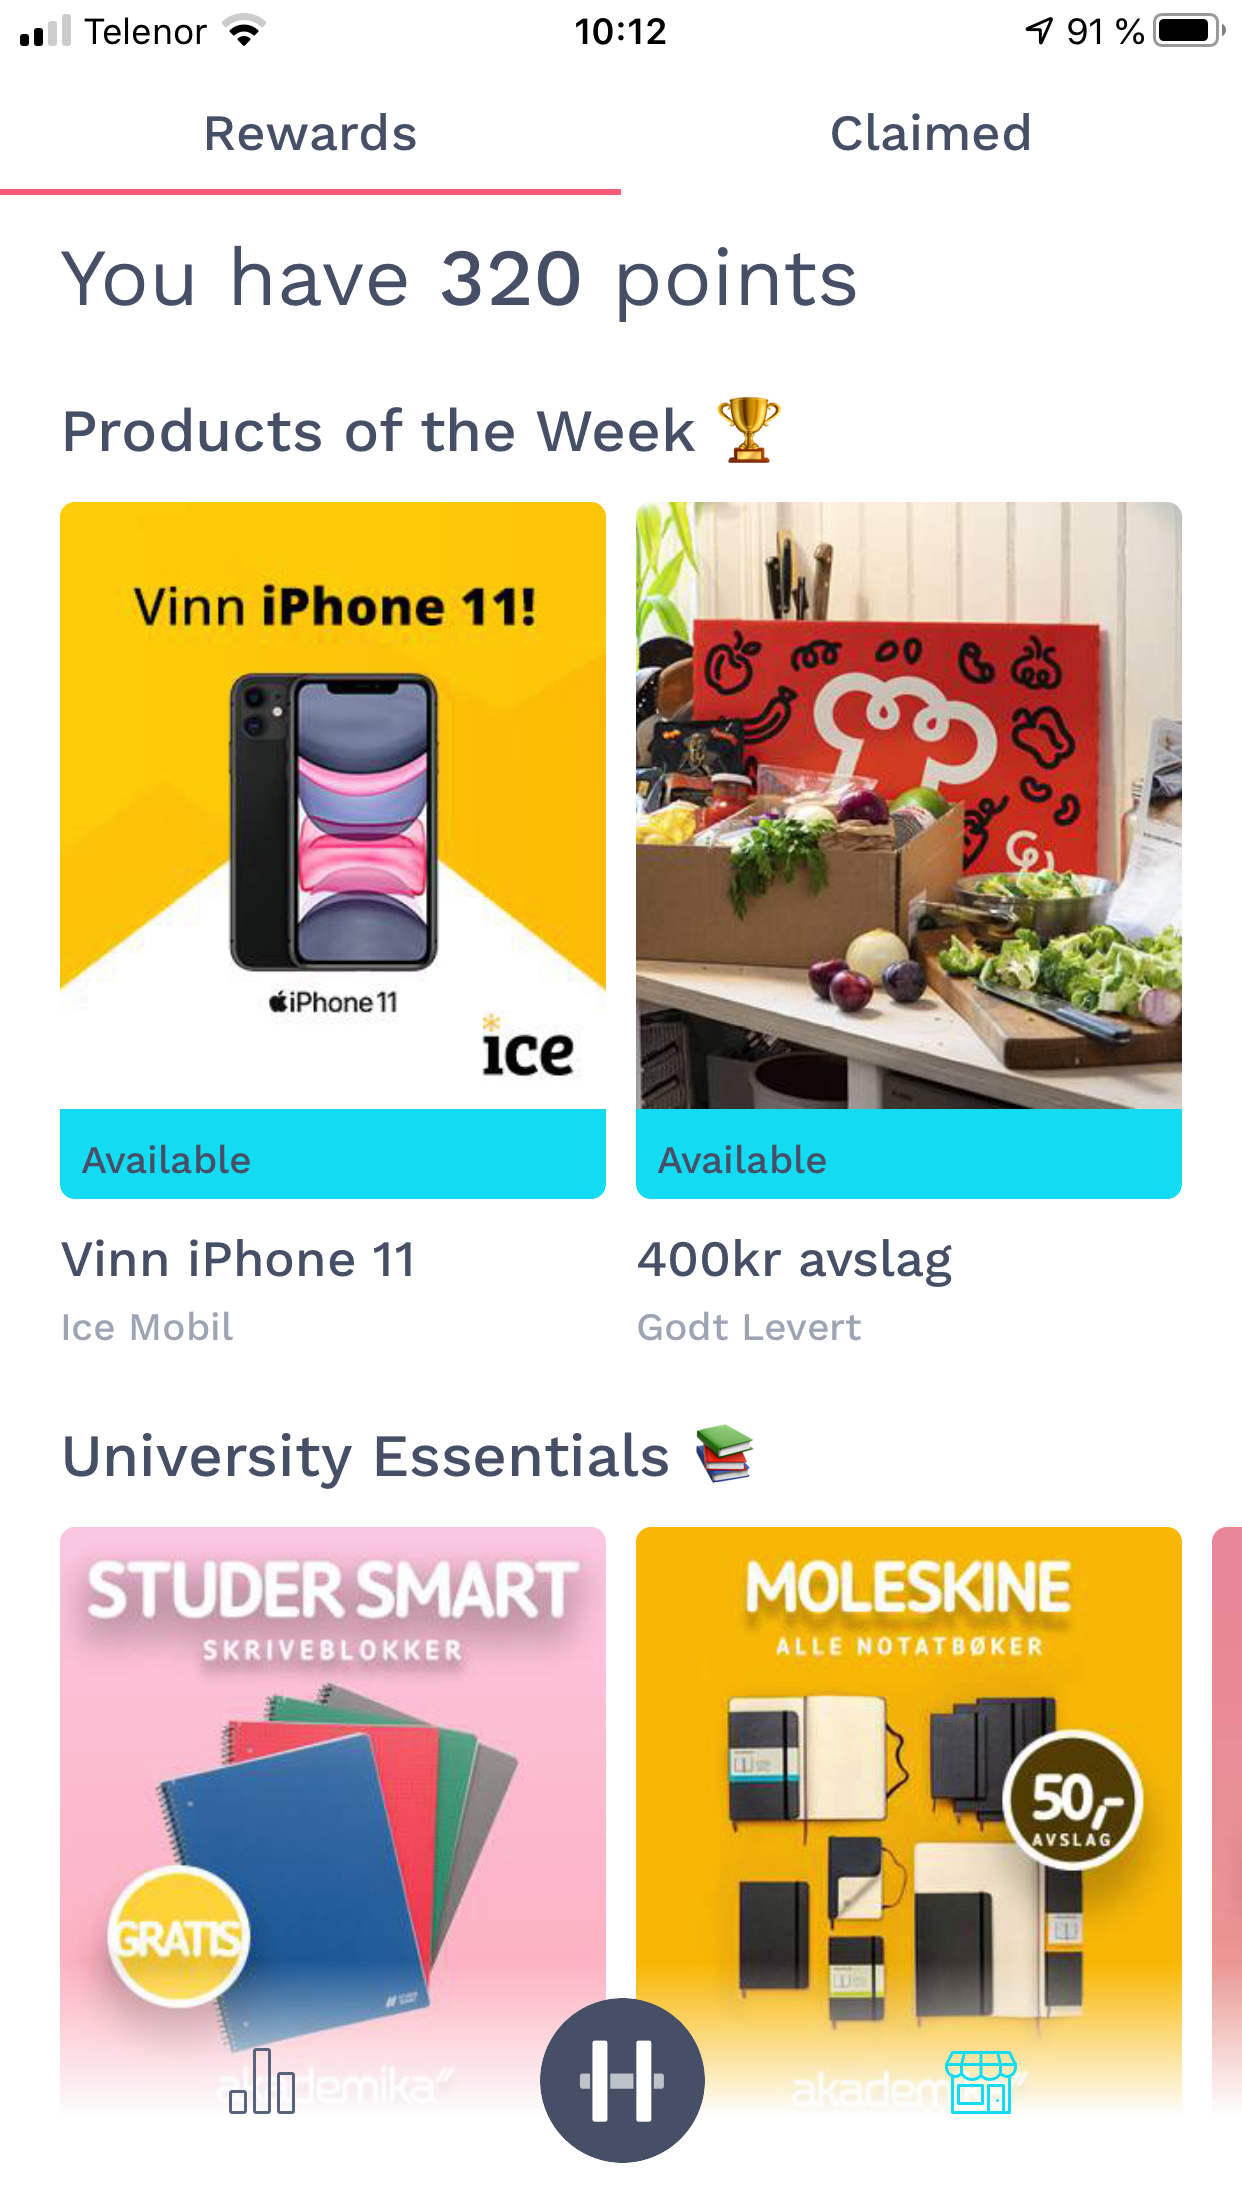
\includegraphics[width=.75\textwidth]{Images/ExistingGames/HoldAppRewards.png}
      \captionof{figure}{Choices of rewards in Hold.}
      \label{fig:hold_reward}
    \end{minipage}
\end{figure}

The application helps users limit distractions through gamification. When users activate the application, a timer starts running (see Figure \ref{fig:hold_timer}). The user is rewarded with ten points for each twentieth minute they are not using their phone. The points can later be exchanged into real-life items such as coffee, food, or discounts, as seen in Figure \ref{fig:hold_reward}. The rewards are the main motivating factor for using the application.

Unlike other games, Hold’s concept is to encourage people not to use their mobile phones. The user can choose to play alone against the environment (PvE) or connect with friends to compare scores, making it more of a competitive game (PvP). The application also lets users connect with nearby friends through Bluetooth, enabling them to focus (collaborate) while boosting their points collectively\citep{wakefield_free_2018}.

Hold is a perfect example of an alternative game with a different concept, where the developers have explored multiple of the game characteristics categories. The game classifies as an alternative primarily for two reasons: It explores alternative game genres by using gamification, rewarding the user points for not using their phone. Furthermore, it uses alternative input sources, primarily Bluetooth, for connecting with nearby friends.

\subsection{Mario Kart Live}
Mario Kart Live is a newly developed augmented reality concept from Nintendo (released 16th October 2020) for its Switch game console. The game is based on the classic Mario Kart game, but with a unique twist: the inclusion of a specially designed racing kart that follows the user’s maneuvers in-game. A live video feed from the racing kart is relayed to the user’s Switch, mapping the virtual track to the user’s home \citep{velazco_race_2020}. The game can be played individually (against AIs) or as a multiplayer game with more than one kart \citep{hashimoto_mario_2020}.

The game is a typical example of how the use of alternative sources for input and output can bring something new to an already familiar game concept. For this Mario Kart game, the alternative twist is the use of a camera for input to produce AR output. Figure \ref{fig:mario_kart_live} shows a poster from the game where you can see the karts racing a user’s home and how the game is presented to the player. 

\begin{figure}[H]
    \centering
    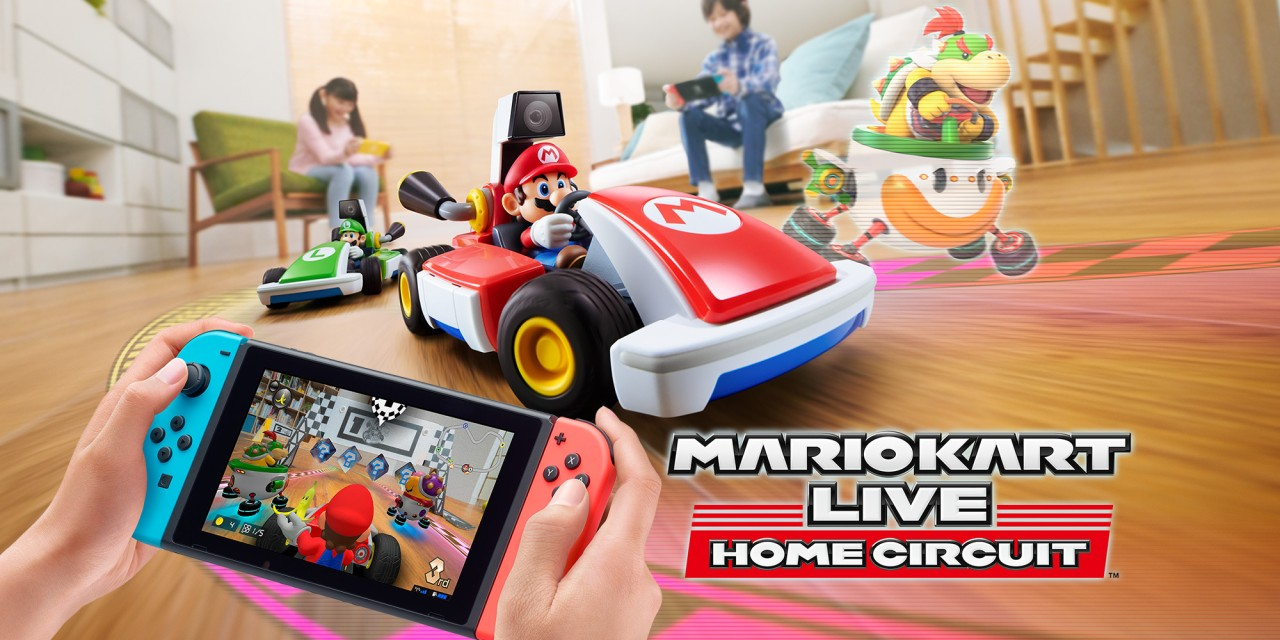
\includegraphics[width=0.8\textwidth]{Images/ExistingGames/MarioKartLive.jpeg}
    \caption{Mario Kart Live poster showing illustrated gameplay.}
    \label{fig:mario_kart_live}
\end{figure}

\subsection{Pokémon Go}
Pokémon Go is another good alternative game example, published and developed by Niantic for iOS and Android. The game was launched in 2016 and quickly became one of the most popular mobile games of all time \citep{grubb_pokemon_2016}. The concept is an extension of the classic Pokémon game found on multiple of Nintendo's handheld devices.

\begin{figure}[H]
    \begin{minipage}{.48\textwidth}
      \centering
      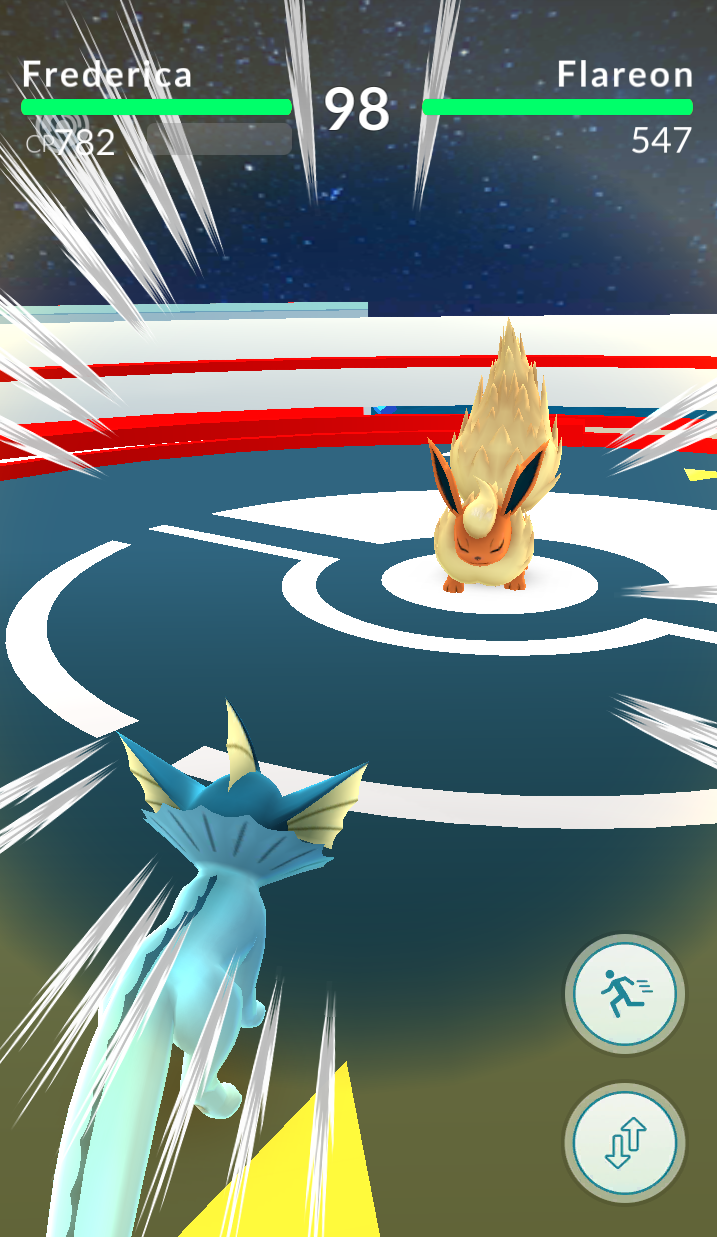
\includegraphics[width=.8\textwidth]{Images/ExistingGames/PokemonGoBattle.png}
      \captionof{figure}{Screenshot of an ongoing battle in Pokémon Go.}
      \label{fig:pokemon_go_battle}
    \end{minipage}
    \hspace{0.5cm}
    \begin{minipage}{.48\textwidth}
      \centering
      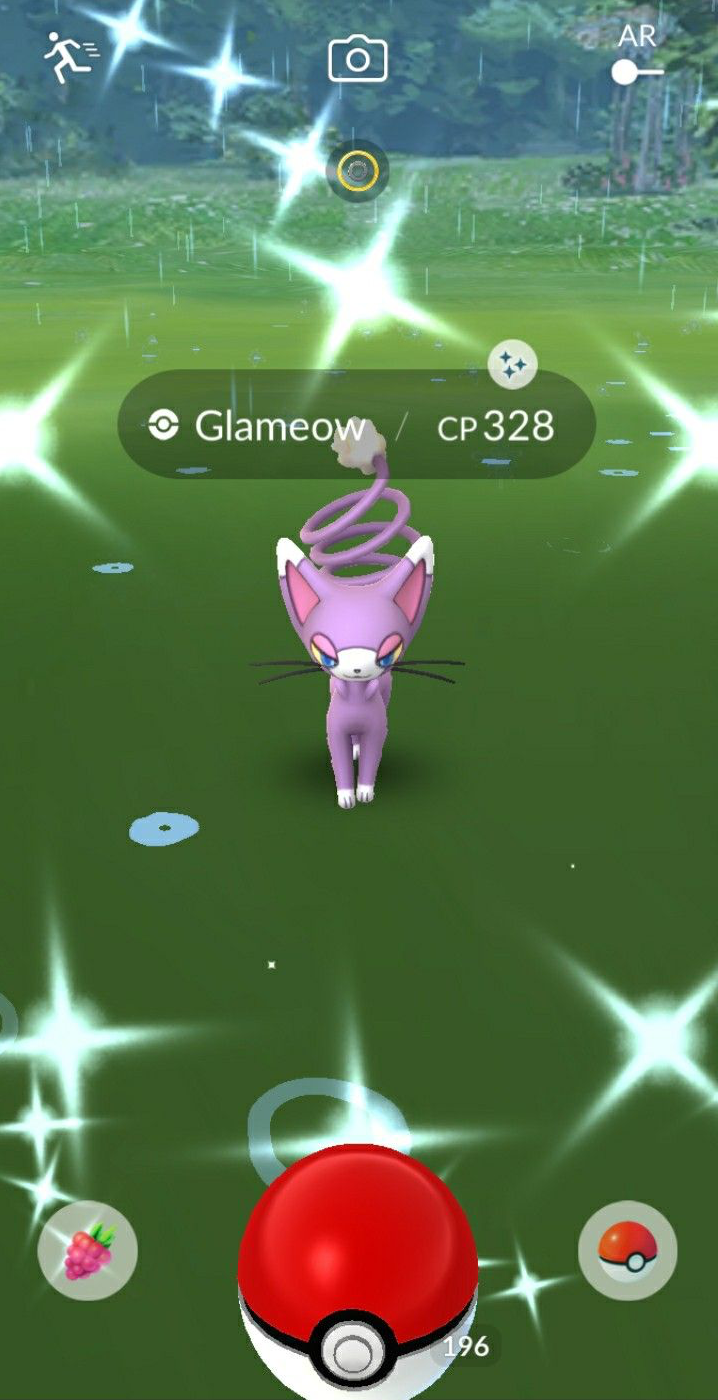
\includegraphics[width=.7\textwidth]{Images/ExistingGames/PokemonGoCatch.png}
      \captionof{figure}{Typical screenshot of gameplay in Pokémon Go.}
      \label{fig:pokemon_go_catch}
    \end{minipage}
\end{figure}

The concept is similar to the previous Pokémon games but utilizes AR and location determination (GPS) to find and catch Pokémons. The player needs to move around in the real world to play the game. Battles between Pokémons (to increase combat points and get prices) can happen at specific places known as Pokémon Gyms. These spots correspond to real-world points of interest (POI) such as parks and tourist attractions \citep{bastow_pokestops_2016}. There are also additional important POI in the game, such as PokéStops and Nests. Figure \ref{fig:pokemon_go_battle} is an in-game screenshot where you can see a typical Pokémon battle, while Figure \ref{fig:pokemon_go_catch} shows a screenshot of gameplay while catching a Pokémon.

The game is an alternative game as it explores uncommon input and output sources such as camera, GPS, and AR. The game is also classified as a pervasive game because the player experience is extended to the real world. A study on \textit{The Pikachu Effect} reveals that the magnitude of Pokémon Go players experience both physical and social benefits from the pervasive game\citep{kaczmarek_pikachu_2017}. Pokémon Go is an excellent example of how alternative games can become very successful.

\subsection{Just Dance Now}
Just Dance Now is an alternative game produced by Ubisoft, launched in 2014 \citep{fandom_just_2020}. The game is an addition to the Just Dance franchise, where the concept is to pick a song from the catalog and follow the moves of the on-screen character, see Figure \ref{fig:just_dance_now_pc}. 

Just Dance Now distinguishes itself from the other games of this type by being more available because it does not require a dedicated gaming console. It can be played using an iOS or Android-based smartphone as the controller and a large screen connected to the internet, such as AppleTV, Chromecast, or a computer \citep{ubisoft_general_2020}. The player's smartphone is used as a movement tracker, and the large screen displays the dance moves they should perform. Multiple players can join the same game and dance together, competing, trying to get the highest score.

\begin{figure}[H]
    \begin{minipage}[t]{.65\textwidth}
        \centering
        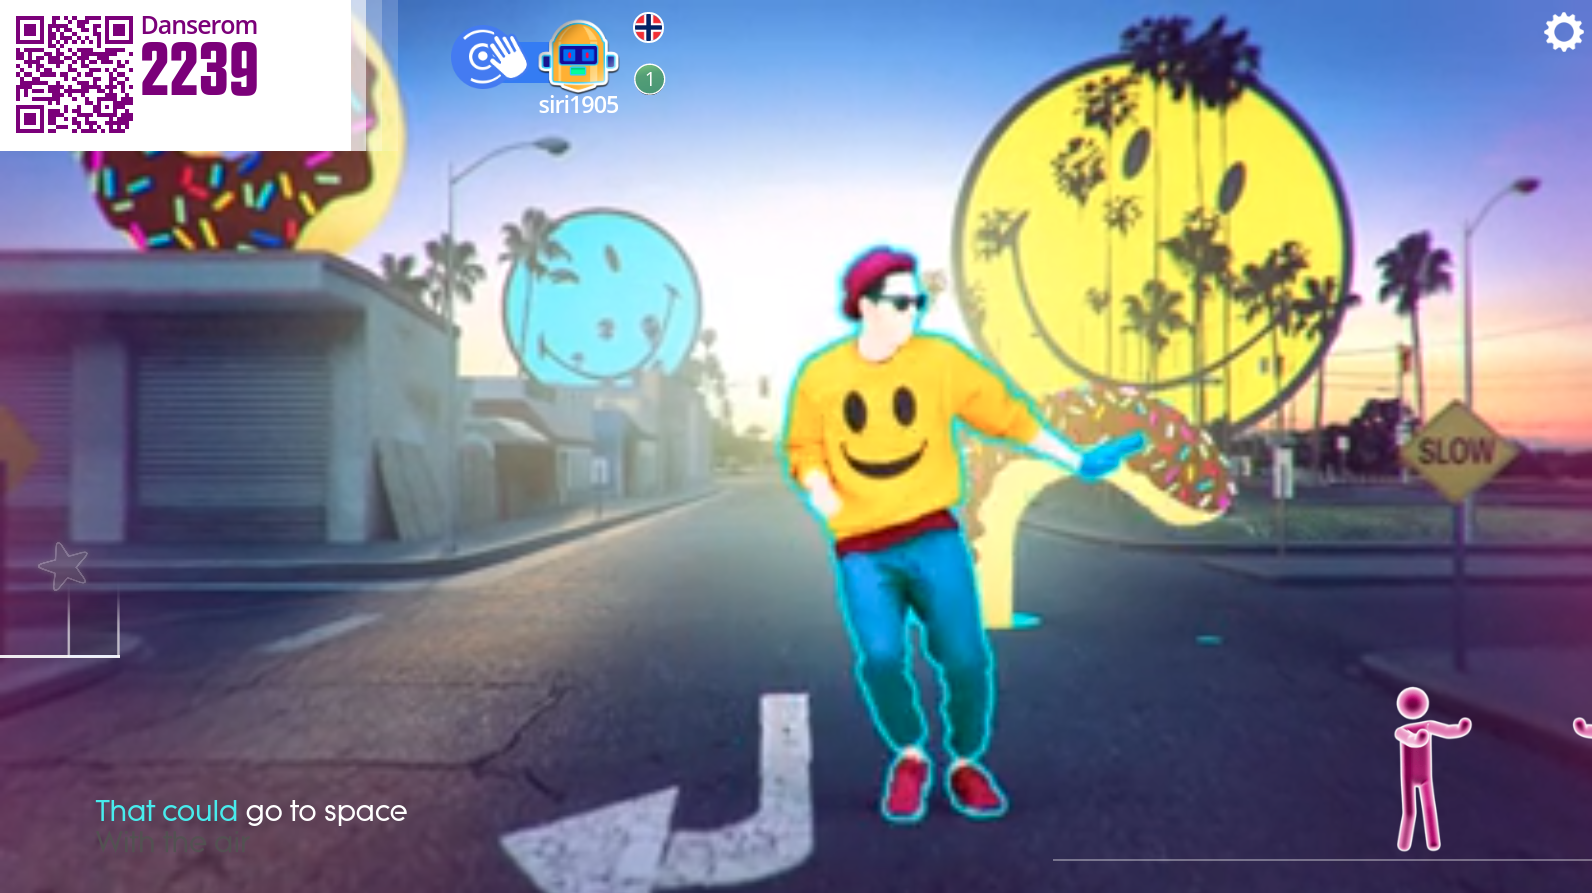
\includegraphics[width=\textwidth]{Images/ExistingGames/JustDanceNow_Pc.png}
        \caption{Just Dance Now screenshot from the computer display.}
        \label{fig:just_dance_now_pc}
    \end{minipage}
    \hspace{0.5cm}
    \begin{minipage}[t]{.35\textwidth}
        \centering
        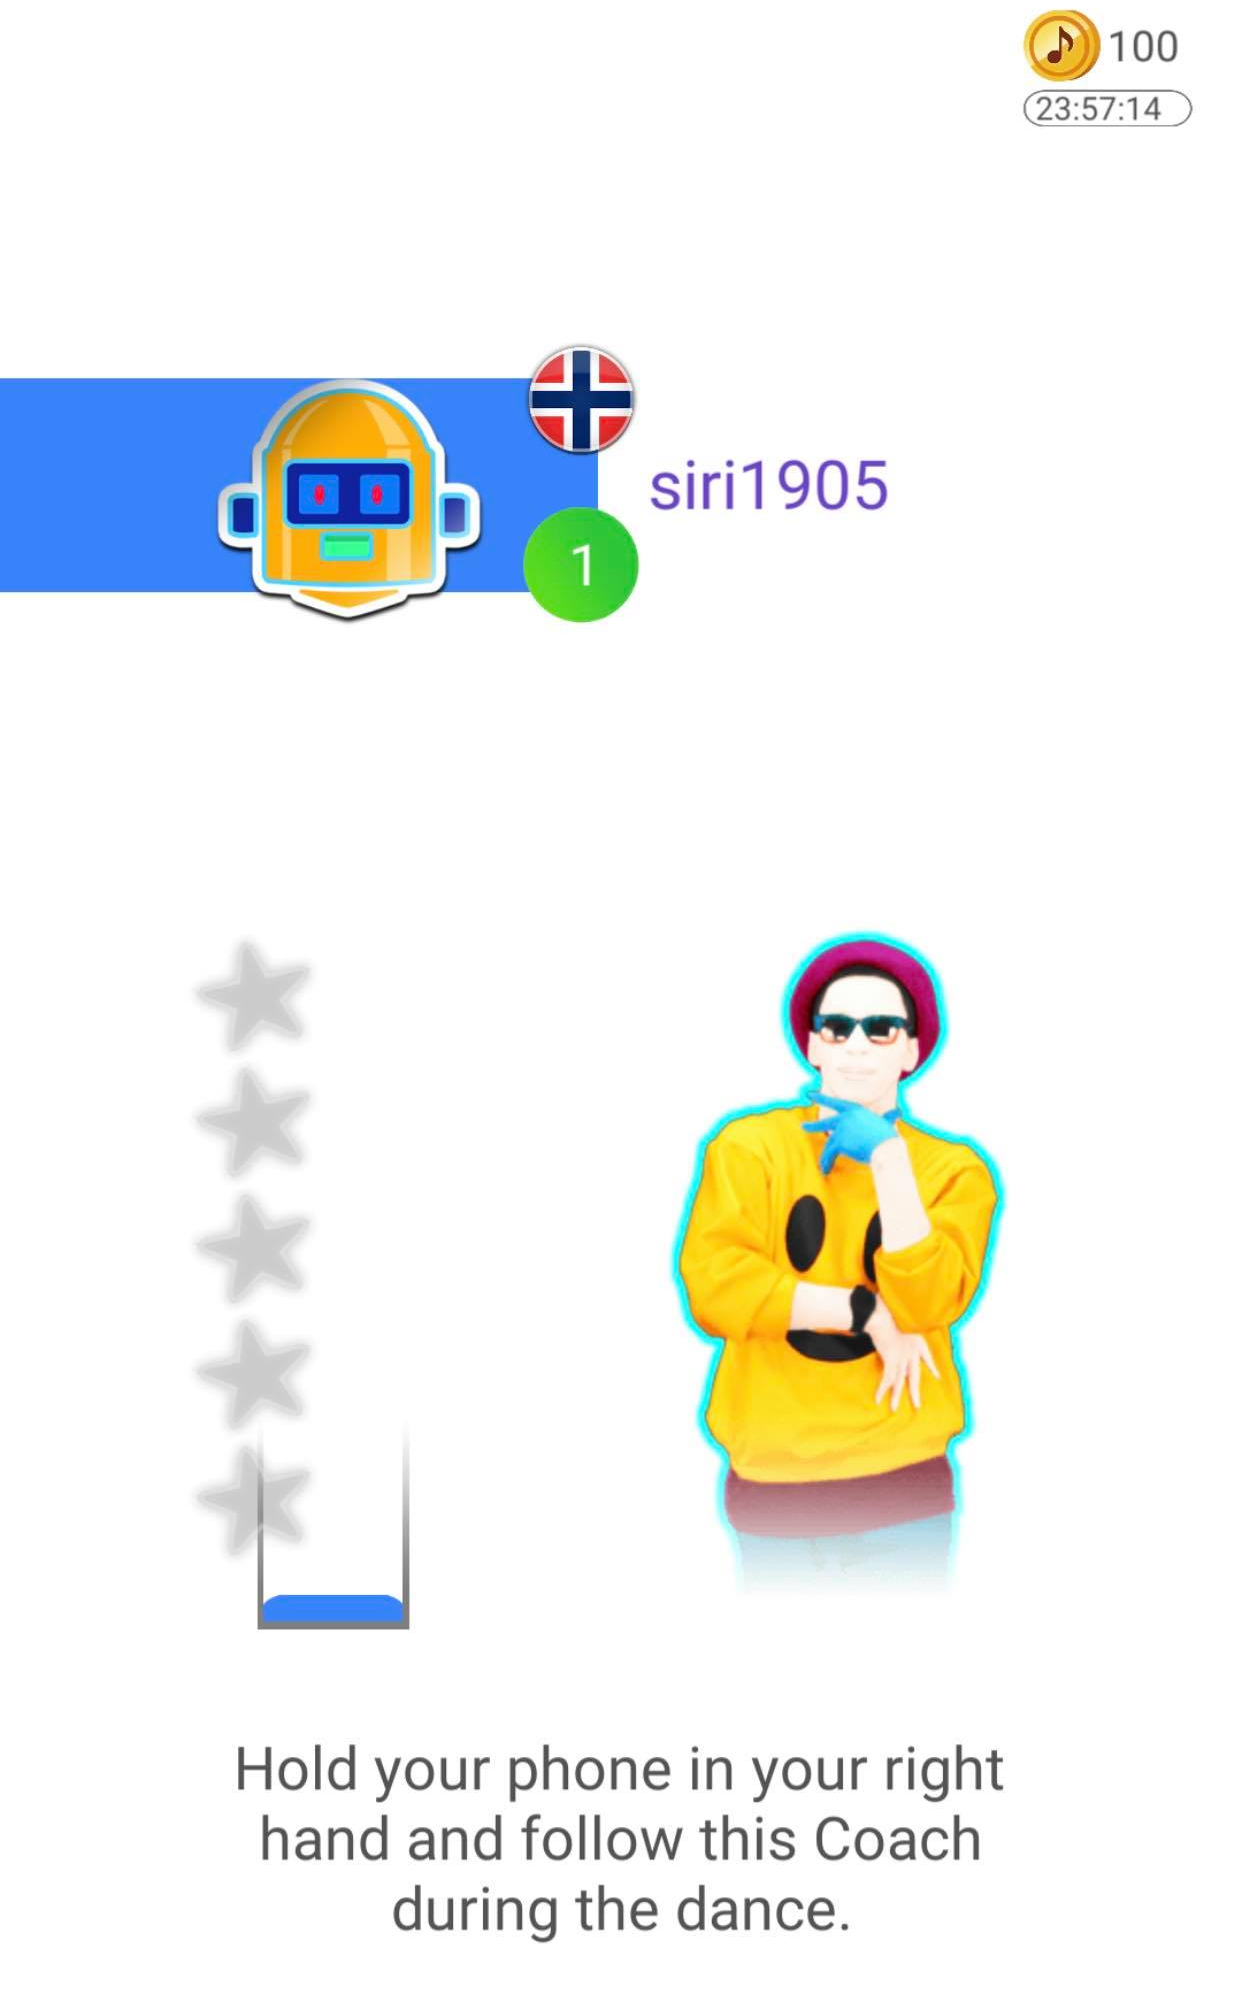
\includegraphics[width=0.8\textwidth]{Images/ExistingGames/JustDanceNow_Mobile.png}
        \caption{Just Dance Now screenshot from a smartphone that is used as a movement controller.}
        \label{fig:just_dance_now_mobile}
    \end{minipage}
\end{figure}

The main reason this game can be seen as an alternative game is based on the use of the player’s mobile phone as a movement tracking device, as seen in Figure \ref{fig:just_dance_now_mobile}. Based on the sensors’ measurements in the player’s phone, the game determines whether or not the player is doing the dance moves well.

The interaction form is another reason why this game is an alternative game. The game is an example of a multi-modal exergame, where all players in one game use the same large screen to see the moves they need to perform in order to earn points. A recent study on the use of exergames in physical education in primary schools, revealed that Just Dance Now had positive effects on students performance, engagement, and motivation for physical activity\citep{quintas_psychological_2020}. This concept can also be described as a “Multiplayer On One Screen Entertainment System” (MOOSES), presented in Chapter \ref{chap:what_is_alternative}. 
        
\subsection{Guitar Hero}
Guitar Hero is a series of games initially developed for PlayStation 2 in 2005. The game series later expanded to multiple other game platforms, including Xbox 360 and Nintendo Wii. The game concept is based on simulation and gamification of playing guitar, using a custom-developed guitar controller (see Figure \ref{fig:guitar_hero_controller}). The player tries to match the in-game “notes” with buttons on the guitar controller, resulting in a score coherent with the number of notes hit. Songs available to choose from vary between different games, but generally, they belong to the genre of rock \cite{metacritic_guitar_2020}. Figure \ref{fig:guitar_hero_controller} shows a screenshot example from playing the game in single-player mode. 

One of the categories of alternative game characteristics is input. As per the definition (in Chapter \ref{chap:what_is_alternative}), a game using alternative input sources can be classified as an alternative game. Guitar Hero is a typical example of such a game because it depends on a custom-designed controller for playing. Additionally, the use of gamification as the game genre is another reason why Guitar Hero can be defined as an alternative game. The main concept of the game can be viewed as gamification of playing guitar.

\begin{figure}[H]
    \begin{minipage}{.35\textwidth}
        \centering
        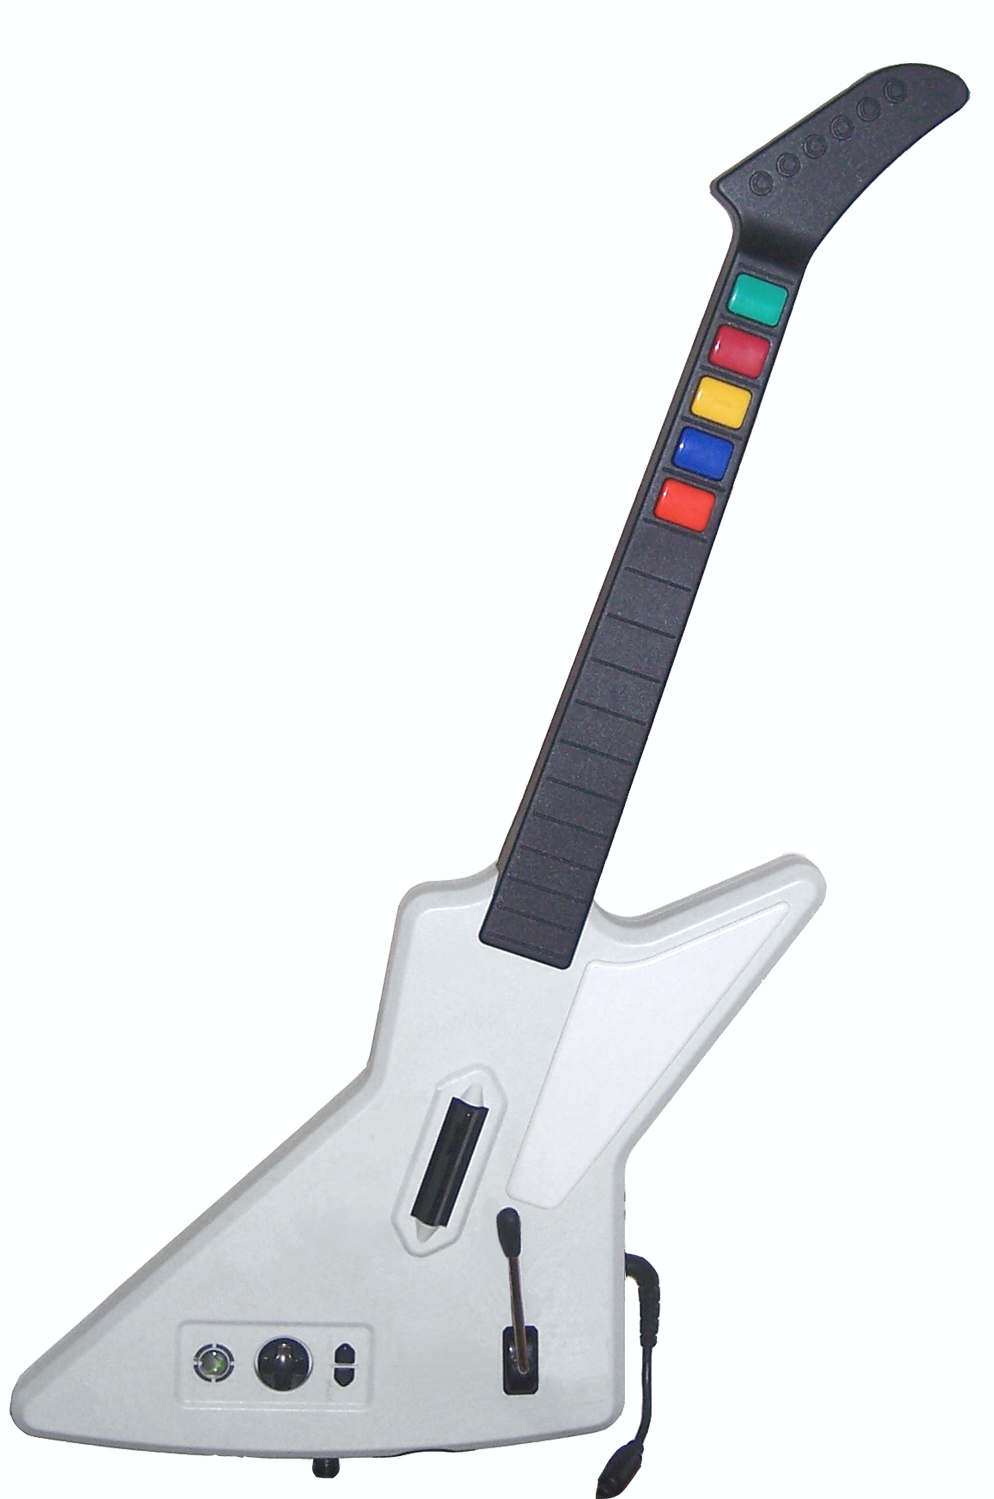
\includegraphics[width=0.9\textwidth]{Images/ExistingGames/GuitarHeroController.png}
        \caption{A Guitar Hero controller.}
        \label{fig:guitar_hero_controller}
    \end{minipage}
    \hspace{0.5cm}
    \begin{minipage}{.65\textwidth}
        \centering
        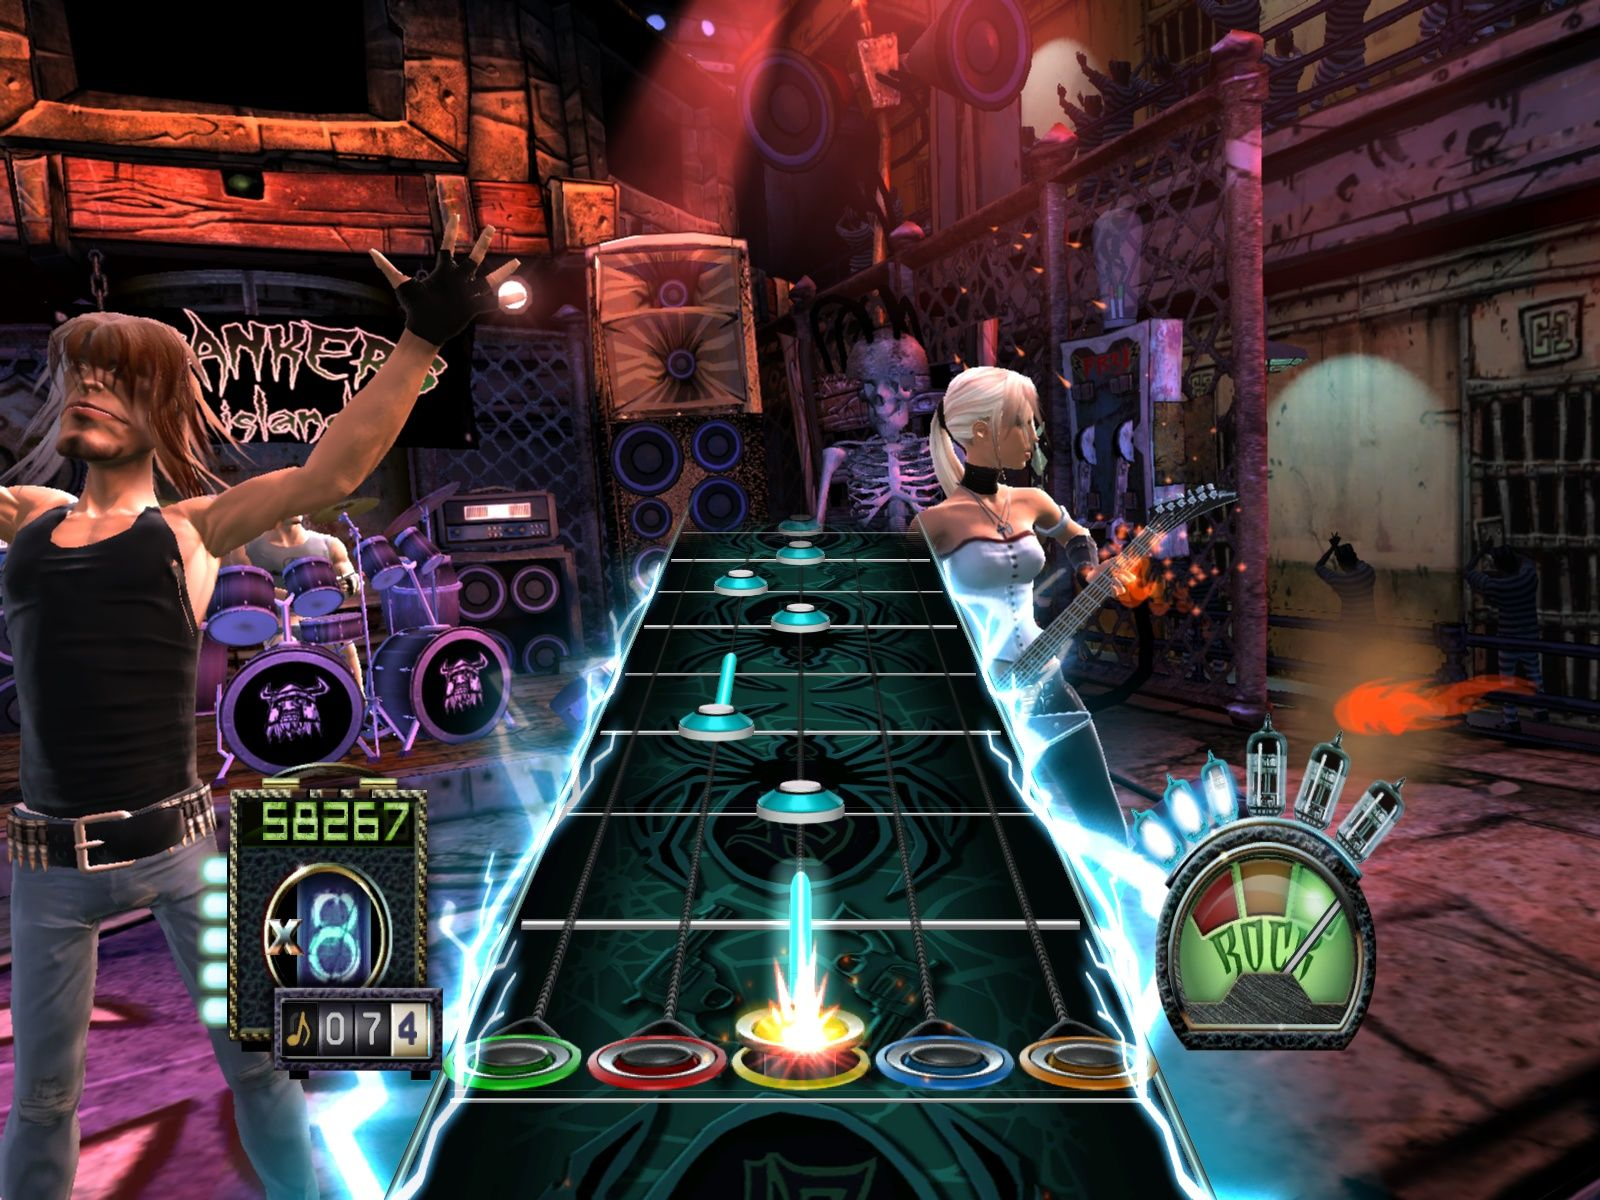
\includegraphics[width=0.9\textwidth]{Images/ExistingGames/GuitarHeroScreenshot.jpg}
        \caption{Screenshot from Guitar Hero gameplay.}
        \label{fig:guitar_hero_screenshot}
    \end{minipage}
\end{figure}
        
\subsection{Wii Fit}
Wii Fit is an exercise game (exergame) created by Nintendo that launched in 2007 \citep{imdb_wii_2020}. The game is only available on Nintendo Wii and requires a unique controller in addition to the regular Wii controller. Wii Fit is a collection of minigames that combine the two domains of health and entertainment. The game has four main exercise categories to choose from; strength training, aerobics, yoga, and balance \citep{ign_wii_2008}.

\begin{figure}[H]
    \centering
    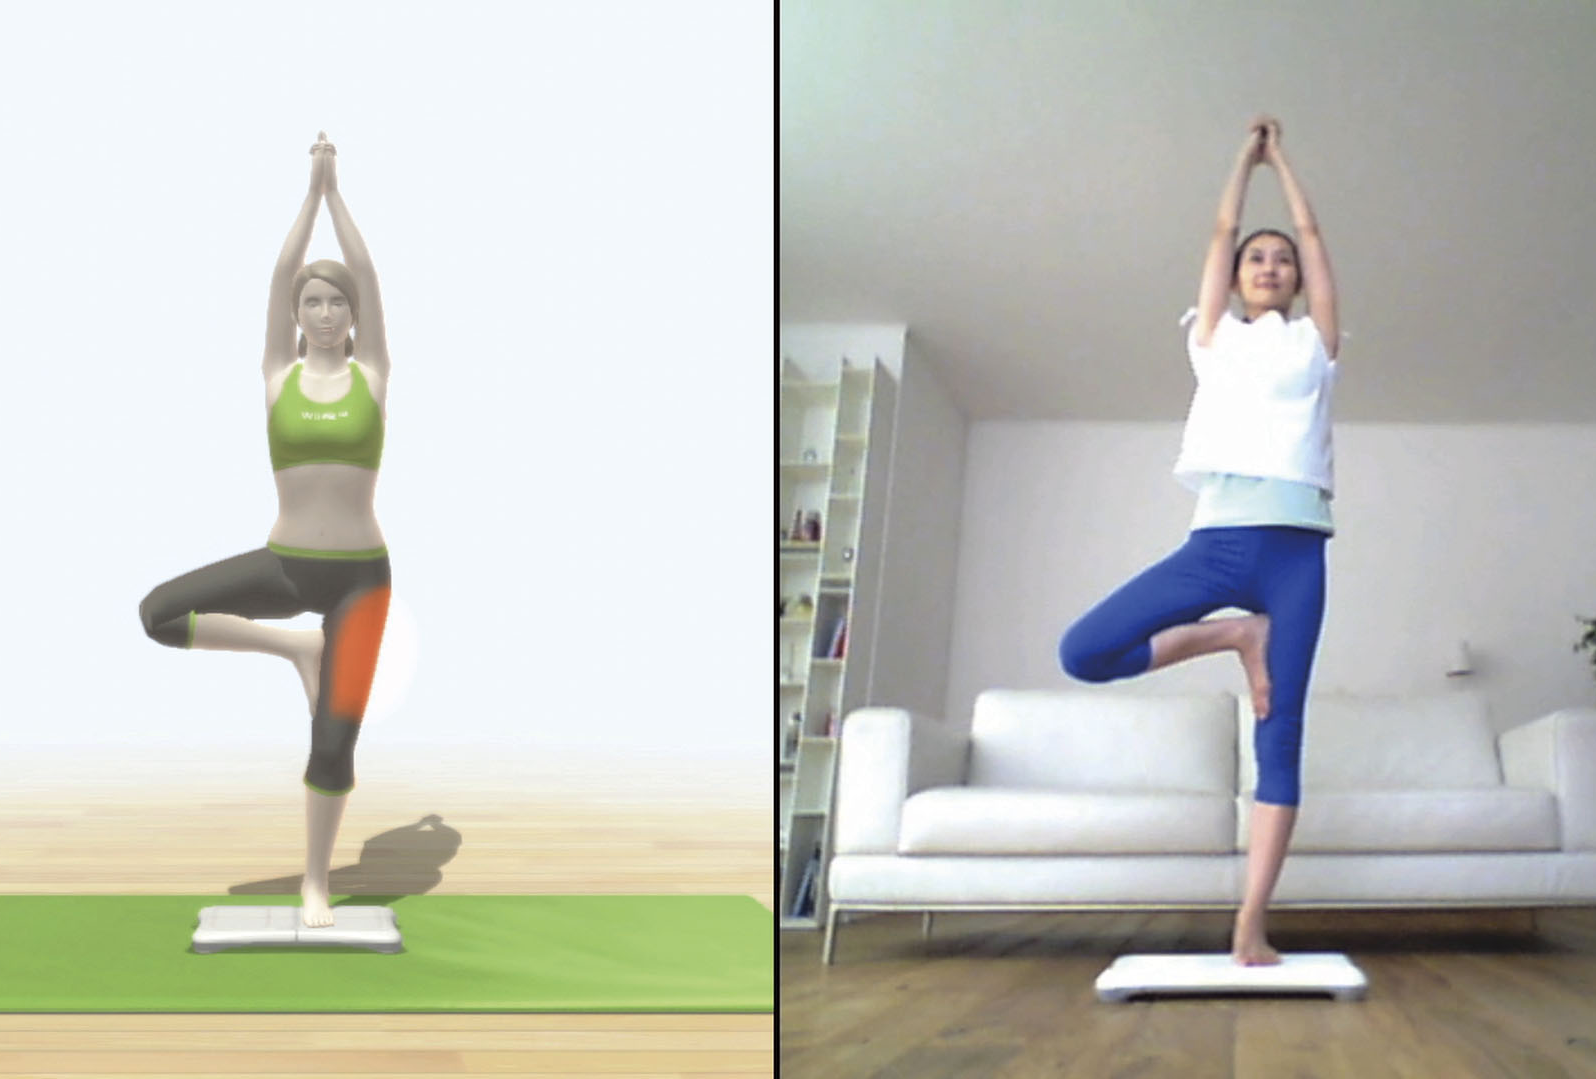
\includegraphics[width=0.75\textwidth]{Images/ExistingGames/WiiFit_Pose.png}
    \caption{A person doing yoga exercise alongside an in-game avatar.}
    \label{fig:wii_fit_pose}
\end{figure}

The additional controller is called the Wii Balance Board \citep{ign_wii_2008} and is one reason this game can be categorized as alternative. The board’s purpose is to track the user's movement and translate it to the user’s in-game avatar, as seen in Figure \ref{fig:wii_fit_pose}. The idea behind the board was drawn from the bathroom weight, and it consists of four weight sensors; one in each corner. The controller connects to the console through Bluetooth, where it calculates the user's movement in real-time \citep{jacquot_how_2010}. Based on the user’s movement, the game gives feedback on how the exercise is going, as seen in Figure \ref{fig:wii_fit_pushup}.

In addition to the alternative input, Wii Fit is also a gamification concept of doing exercise. The game’s goal is to create a fun way of getting in shape from a user’s own home. Nintendo brings a comprehensive set of games that are engaging for the entire family with individual progress so all players can compare themselves against each other.

Wii Fit was originally designed as an interactive health and fitness experience for the general public. However, the benefits of Wii Fit have been studied in many clinical settings, such as in multiple sclerosis patients and stroke patients\citep{tripette_contribution_2017}. A 2011 study of the health and wellness benefits of Wii Fit on university students, revealed a significant change in body mass index, weight, and intrinsic and total motivation for its participants\citep{jacobs_wii_2011}.

\begin{figure}[H]
    \centering
    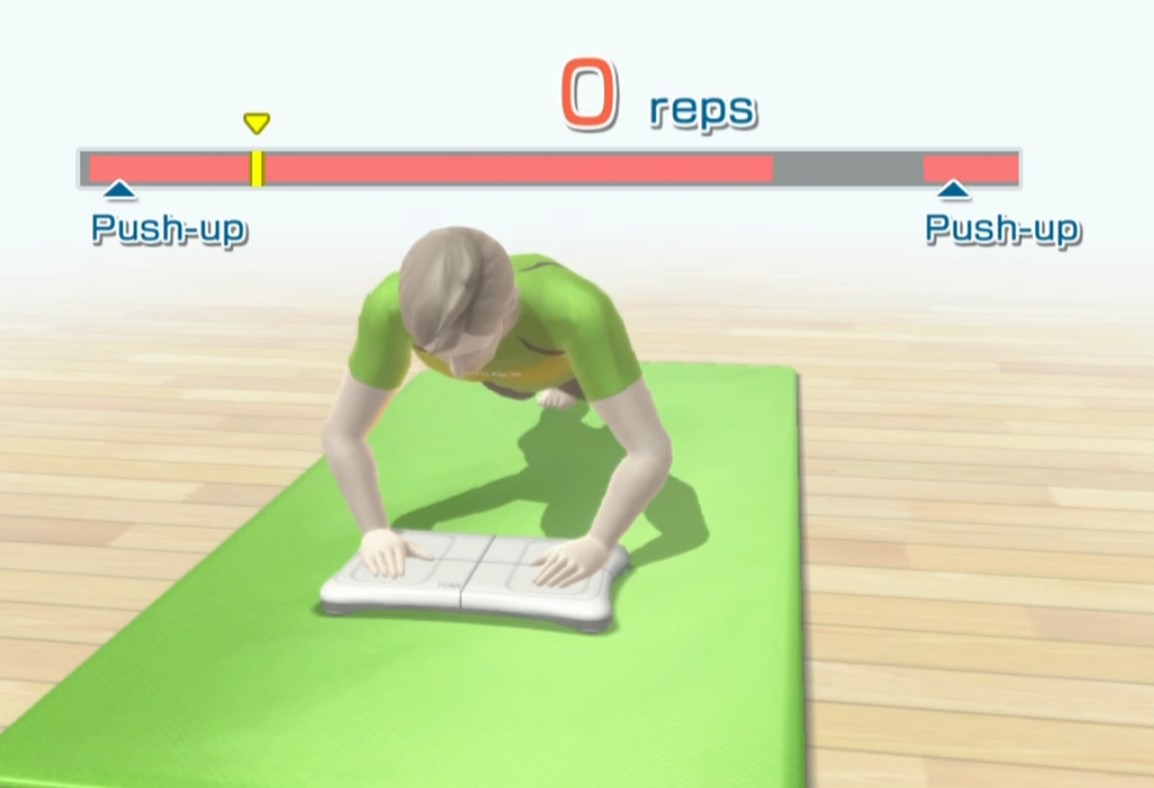
\includegraphics[width=0.75\textwidth]{Images/ExistingGames/WiiFit_Pushup.jpg}
    \caption{Screenshot of the in-game avatar using the board to track push-ups.}
    \label{fig:wii_fit_pushup}
\end{figure}

\subsection{Mosquito Mania}
Mosquito Mania is a game concept developed at NTNU in connection with a music technology bachelor thesis in 2012. The game was developed as an attempt to create a new way of entertaining people by using audio stimulation together with concepts from game development.

The primary purpose of the game is to kill as many mosquitos as possible within 60 seconds. An 8-32 array of speakers is positioned in a circle around the player, emitting mosquito sounds in a 2-dimensional space, as seen in Figure \ref{fig:mosquito_mania_anonym}. The player is then assigned the task to try and kill the mosquitos using a custom made gun-like controller, measuring the direction it is pointed. A microcontroller combined with an accelerometer, compass, and gyroscope is mounted on the controller. Though the game primarily focuses on audio, the game has a dashboard for game statistics and scoreboard (see Figure \ref{fig:mosquito_mania_dashboard})

The game is alternative for multiple reasons. First of all, it uses an alternative input source, i.e., the custom controller for playing. This special controller could by itself contributed to categorize the game as alternative. However, the primary reason for Mosquito Mania to be an alternative game is the unusual approach of using audio as the primary output source. Regular games typically combine sounds and music as a secondary output source in addition to visual feedback. The game concept is unique, and by removing the visual aspect, a new twist is introduced to the game. Even though the game was not developed for any special target groups, it became immensely popular among people with visual impairment \citep{gran-jansen_mosquito_2020}.

\begin{figure}[H]
    \begin{minipage}[t]{.5\textwidth}
        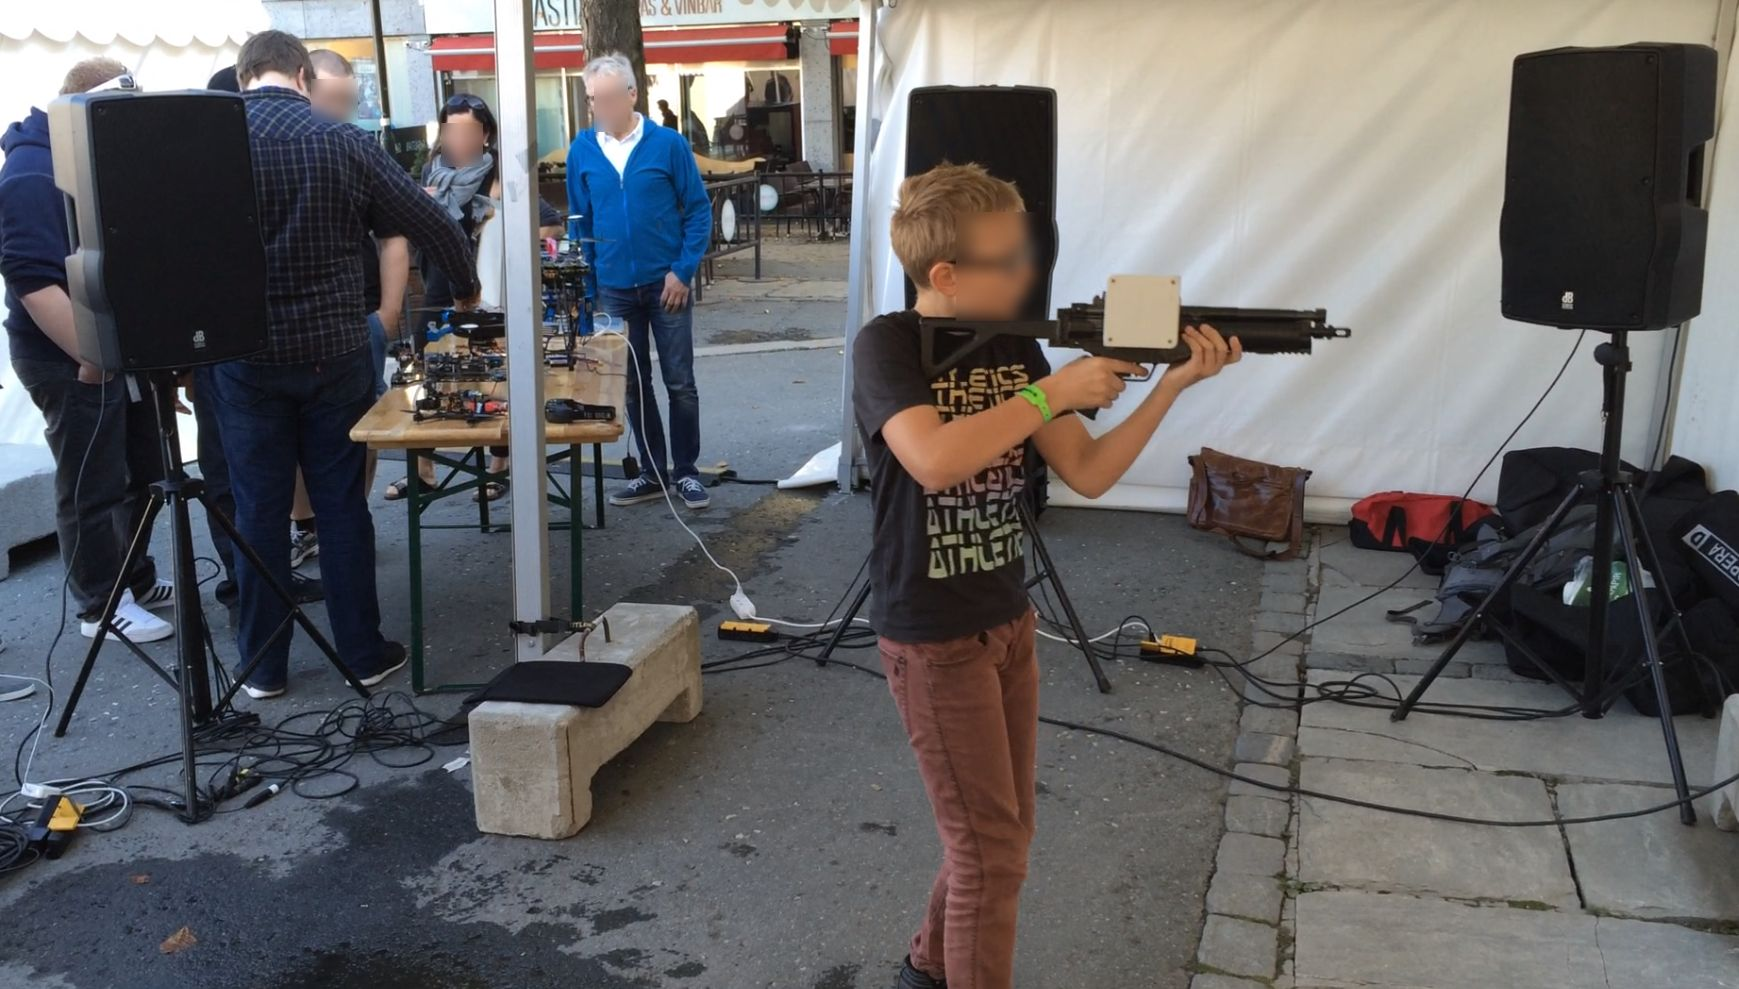
\includegraphics[width=\textwidth]{Images/ExistingGames/MosquitoMania_anonym.jpg}
        \caption{The player is surrounded by speakers that emit mosquito sounds. The handheld gun is used to aim at the imaginary mosquito to score points.}
        \label{fig:mosquito_mania_anonym}
    \end{minipage}
    \hspace{0.05\textwidth}
    \begin{minipage}[t]{.5\textwidth}
        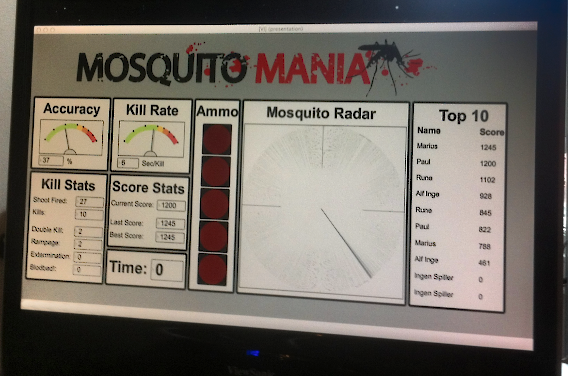
\includegraphics[width=0.87\textwidth]{Images/ExistingGames/MosquitoMania_Dashboard.png}
        \caption{The game’s dashboard shows game statistics and a top 10 scoreboard.}
        \label{fig:mosquito_mania_dashboard}
    \end{minipage}
\end{figure}

\biblio % Needed for referencing to working when compiling individual subfiles - Do not remove
\end{document}